\begin{figure}[H]
    \centering
    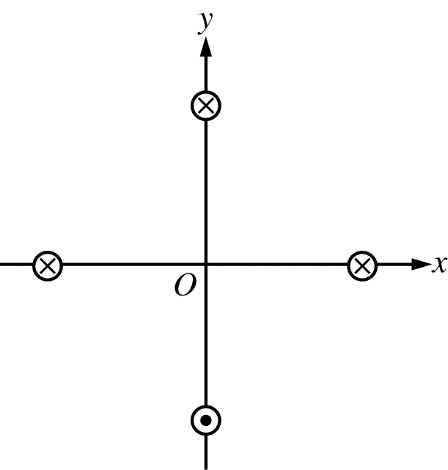
\includegraphics[scale=0.4]{images/img-014-035.png}
\end{figure}

% Multiple Choice Question 32
\begin{questions}\setcounter{question}{31}\question
Four long, straight wires are perpendicular to the $x y$-plane. Each wire is the same distance from the origin $O$, as shown in the figure above. The wires have equal currents that are in the directions shown. Which of the following best represents the direction of the net magnetic field, if any, at the origin due to the four currents?

\begin{choices}
\choice \adjustbox{valign=t}{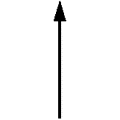
\includegraphics[scale=0.3]{images/img-014-036.png}}
\choice \adjustbox{valign=t}{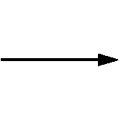
\includegraphics[scale=0.3]{images/img-014-037.png}}
\choice \adjustbox{valign=t}{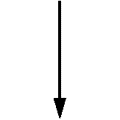
\includegraphics[scale=0.3]{images/img-014-038.png}}
\choice \adjustbox{valign=t}{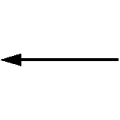
\includegraphics[scale=0.3]{images/img-014-039.png}}
\choice Undefined because the net field is zero.
\end{choices}\end{questions}
